\documentclass{beamer}
%\usetheme{Ilmenau}
%\usetheme{Berlin}
%\usetheme{Montpellier}
%\usetheme{CambridgeUS}
\usetheme{Hannover}
%\usetheme{Singapore}

\usepackage[utf8]{inputenc}
\usepackage[T1]{fontenc}
\usepackage{lmodern}

\usepackage{graphicx} 
\usepackage{amsmath}
\usepackage{chronology}

\author{Loïc Messal}
\date{20 octobre 2016}
\title{Initiation à \LaTeX}
\institute{Service formation Vertigéo \\ \emph{La formation par les étudiants, pour les étudiants !}}

\AtBeginSection[]{
  \begin{frame}{Sommaire}
  	\small \tableofcontents[currentsection, hideothersubsections]
  \end{frame} 
}

\usepackage[french]{babel}


\begin{document}
\begin{frame}
	\titlepage
\end{frame}

\section*{Table des matières}
\begin{frame}
	\tableofcontents
\end{frame}

\section{Introduction}

\subsection{Comment ça se prononce ?}
\begin{frame}
	\begin{block}{}
		\LaTeX{} se prononce \og{}lah-tech\fg{}.
	\end{block}
\end{frame}

\subsection{À quoi ça sert ?}
\begin{frame}
	\begin{itemize}
		\item Système de composition de haute qualité.
		      \pause
		\item Libre
		      \pause
		\item Open source
		      \pause
		\item Multi plateformes
	\end{itemize}
\end{frame}

\begin{frame}
	\begin{chronology}[5]{1975}{1997}{10cm}[10cm]
		\event{1975}{\color{black}{Unix 6}}	
		\event{1977}{\color{blue}{\TeX}}
		\event{1983}{\color{blue}{\LaTeX} \color{black}{--} \color{blue}Word}
		\event{1984}{\color{black}{Mac OS 1.0}}
		\event{1985}{\color{black}{Windows 1.0}}
		\event{1991}{\color{black}{Linux 0.01-0.1}}
	\end{chronology}
	LaTeX facilite l'utilisation de TeX.
\end{frame}

\begin{frame}
	Utilisé pour la communication et la publication de documents scientifiques.
				
	\begin{block}{Idée fondamentale : }
		Laisser le design du document aux designers de documents.
	\end{block}
	$\implies$ Se concentrer sur l'écriture du document
\end{frame}

\section{Usage}
\subsection{Comment ça marche ?}
\begin{frame}
	\begin{figure}[!ht]
		\begin{center}
			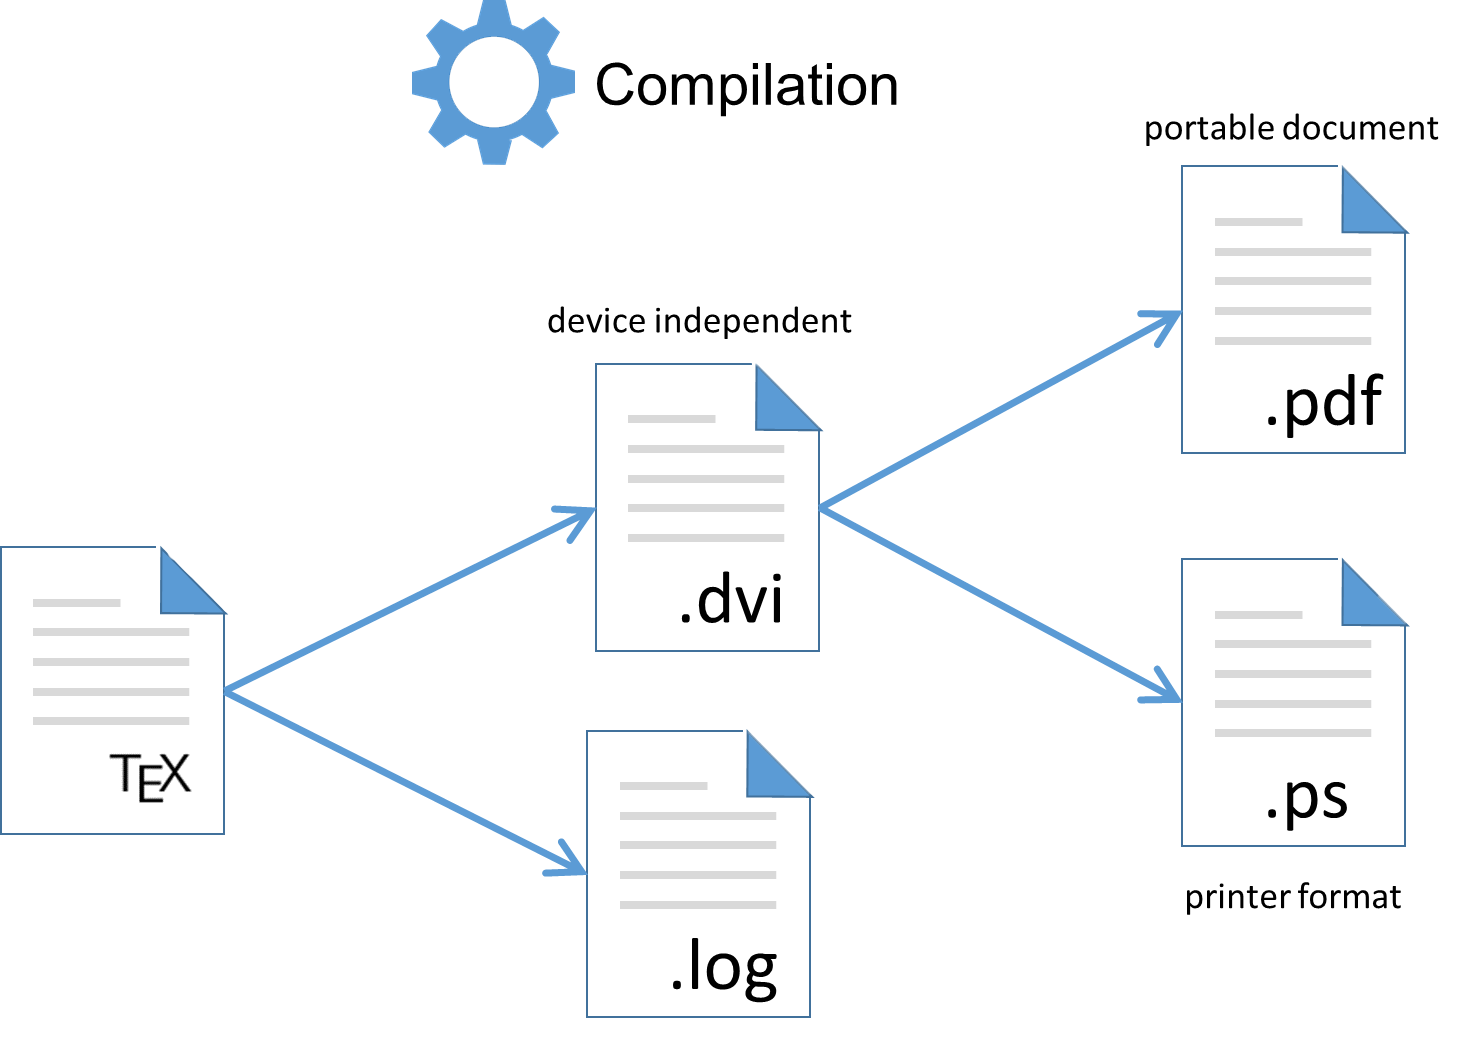
\includegraphics[width=0.60\linewidth, keepaspectratio]{images/compilationLatex.png}
		\end{center}
	\end{figure}
	
	Plusieurs distributions : 
	\begin{itemize}
		\item Linux : texlive
		\item MacOS : mactex
		\item Windows : miktex, protext, texlive
		\item Online : papeeria, overleaf, sharelatex
	\end{itemize}
\end{frame}

\subsection{Comment je m'en sers ?}
\begin{frame}[fragile]
	\LaTeX{} est capricieux. Il faut respecter la structure.
	\begin{center}
		\begin{minipage}{0.5\linewidth}
			\begin{verbatim}
	\documentclass[...]{...}
	
	\usepackage[...]{...}
	
	\begin{document}
			\end{verbatim}
			\vdots
			\begin{verbatim}
	\end{document}
			\end{verbatim}
		\end{minipage}
	\end{center}
\end{frame}

\section{Exemples}
\subsection{La pratique}
\begin{frame}
	\begin{center}
		On commence ?
	\end{center}
\end{frame}
\end{document}